%overview
The system consists of three major parts, the provider on the stm32 board, a Python flask app as a consumer, and the Eclipse Arrowhead framework.
The main objective of the Eclipse Arrowhead framework is to connect the consumer and the provider in a safe and structured way.
The provider is built with C/C++ using ARMs' mbed os, and mainly the mbed-http library. 
\section{System architecture}
\subsection{Services}
The provider offers two services to the consumer. 
The first one is sending the temperature from the LPS22HB temperature and pressure sensor. 
The service URI of this service is /temperature and when performing a GET request the temperature reading will be returned as an integer.
A sequence diagram visualizing how the temperature service is implemented.
\begin{figure}[H]
    \centering
    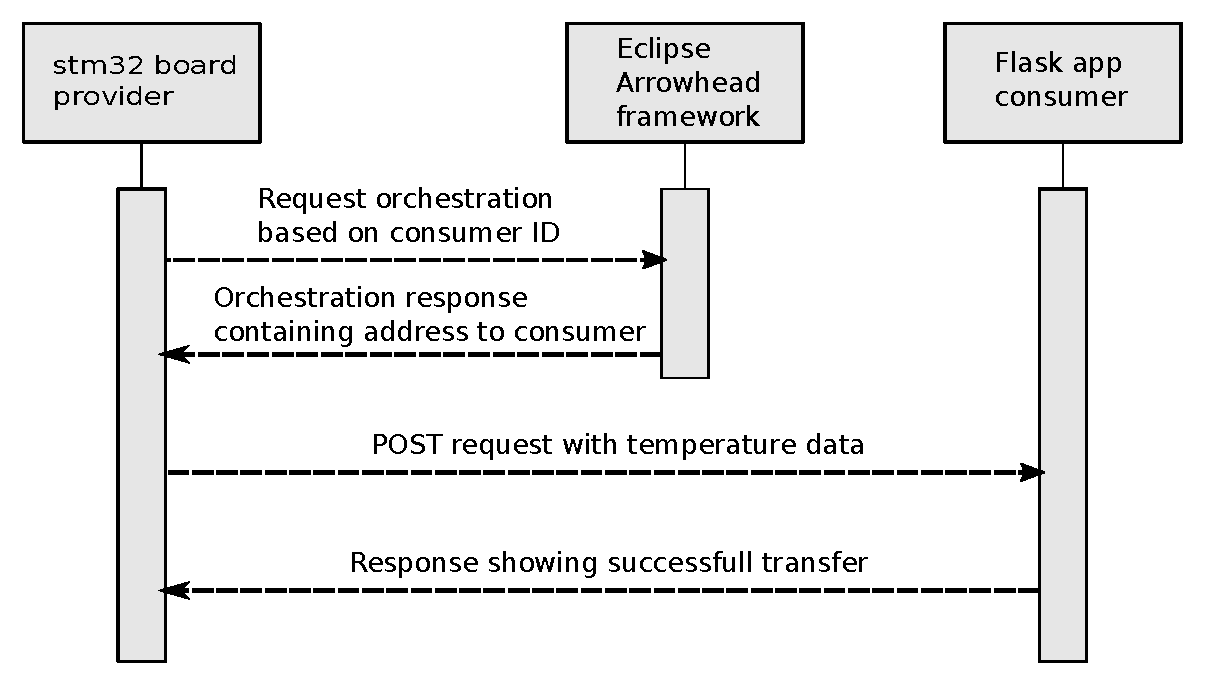
\includegraphics[width=\textwidth]{Pictures/sequence_diagram_consumer.pdf} 
    \caption{Sequence diagram of the process of connecting the consumer and provider through the temperature service.}
    \label{sequence diagram consumer}
\end{figure}
The second one is turning on and off a LED based on the state of that LED.
The service URI of this server is /LED and the desired state of the LED, ON or OFF, is specified in the payload of that call.
It returns the new state of the LED and perform that action on the LED.
A sequence diagram visualizing how the LED service is implemented.
\begin{figure}[H]
    \centering
    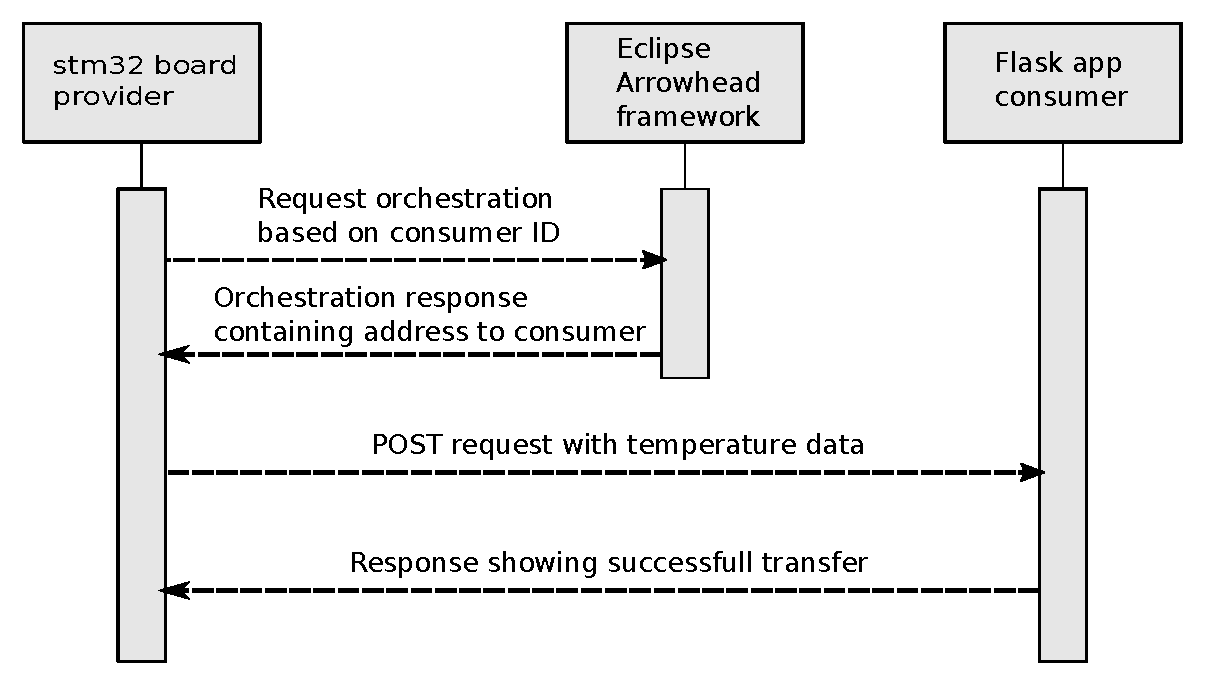
\includegraphics[width=\textwidth]{Pictures/sequence_diagram_consumer.pdf} 
    \caption{Sequence diagram of the process of connecting the consumer and provider through the LED service.}
    \label{sequence diagram consumer}
\end{figure}

\subsection{Sequence of execution}
Since the core systems is dependent on each other, the order of execution of the queries to the database matters a lot.
To have the board act as a part of an Arrowhead system and registering that to the local cloud the following order of execution has to be used.
\begin{itemize}
    \item Register provider.
    \item Register consumer.
    \item Register a service definition.
    \item Add intracloud authorization rules.
    \item Create an orchestration store entry.
    \item Recieve orchestration information based on consumer ID.
\end{itemize}
A sequence diagram visualizing the order of execution in the core systems.
\begin{figure}[H]
    \centering
    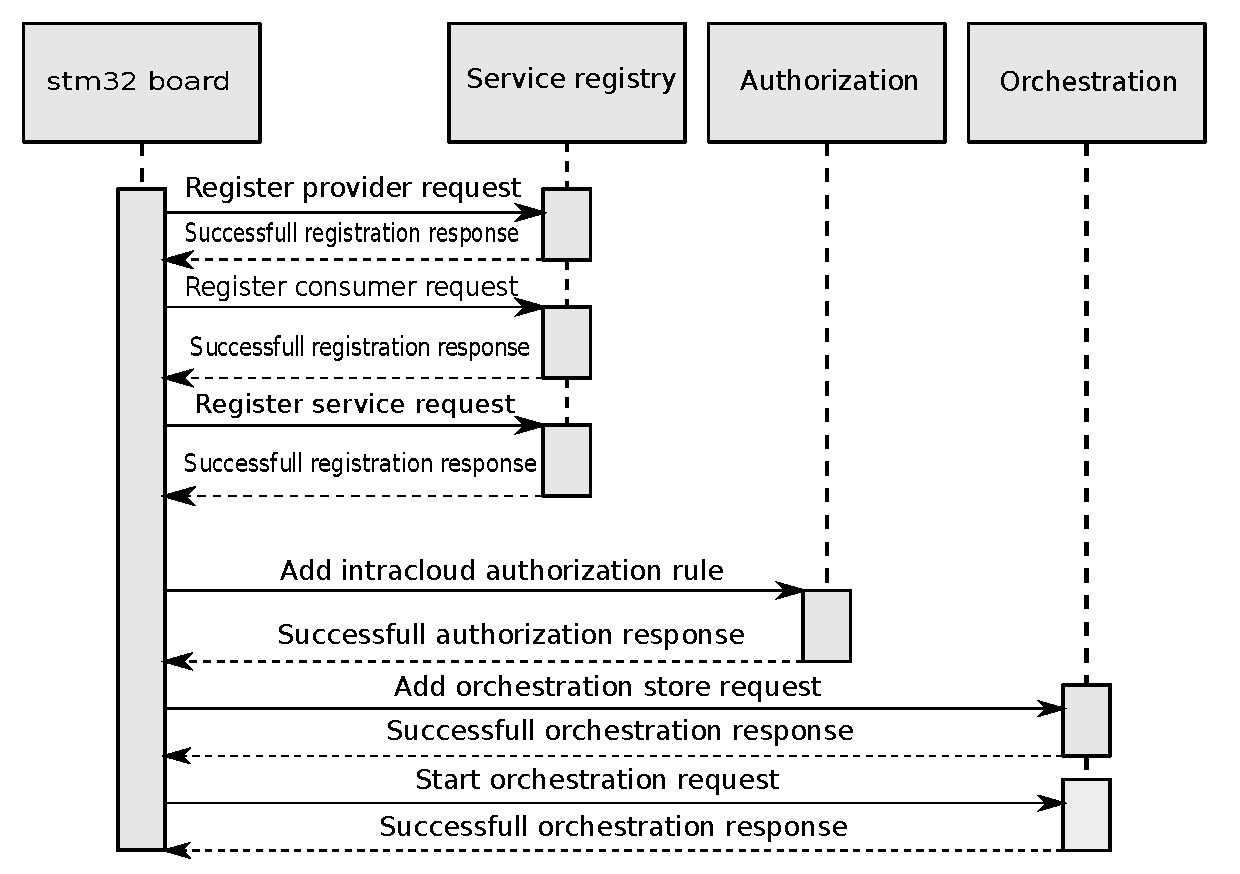
\includegraphics[width=\textwidth]{Pictures/sequence_diagram_total.pdf} 
    \caption{Sequence diagram of the process of using the Eclipse Arrowhead framework.}
    \label{sequence diagram whole process}
\end{figure}

\section{System components}
Based on the architecture described in the previous section it is clear that the software components have two main tasks
\begin{itemize}
    \item Send and recieve information using HTTP POST and GET methods.
    \item Constructing correct JSON strings to act as payload in the POST and GET methods. 
\end{itemize}
\subsection{HTTP post using the mbeb-http library}
The first function performs a HTTP post with a constructed JSON body as payload.
It does that with the help of the network interface object defined in the setup and sends that post to the appropriate URL.
\begin{lstlisting}[style=CStyle]
    std::string http_post_request_with_response(NetworkInterface* _net, std::string url, std::string body)
    {
        HttpRequest *post_request = new HttpRequest(_net, HTTP_POST, url.c_str());
        post_request->set_header("Content-Type", "application/json");
        HttpResponse *post_response = post_request->send(body.c_str(), strlen(body.c_str()));
        if (!post_response) {
            printf("HttpRequest failed (error code %d)\n", post_request->get_error());
            return std::to_string(post_request->get_error());
        }
        printf("\n----- HTTP POST response -----\n");
        std::string response_body = post_response->get_body_as_string();
        delete post_response;
        return response_body;
    }
\end{lstlisting}
\subsection{HTTP get using the mbeb-http library}
The second function is similar to the first one with the main difference that it performs an HTTP get with a JSON payload.
It also uses the network interface to send it to the appropriate URL.
It does that with the help of the network interface object defined in the setup and sends that post to the appropriate URL.
\begin{lstlisting}[style=CStyle]
std::string http_get_request_with_response(NetworkInterface* _net, std::string url)
{
    HttpRequest *get_request= new HttpRequest(_net, HTTP_GET, url.c_str());

    HttpResponse *get_request_response = get_request->send();

    if (!get_request_response) {
        printf("HttpRequest failed (error code %d)\n", get_request->get_error());
        return std::to_string(get_request->get_error());
    }
    printf("\n----- HTTP GET response -----\n");
    std::string response_body = get_request_response->get_body_as_string();
    delete get_request_response;
    return response_body;
}
\end{lstlisting}
\subsection{Constructing appropriate JSON strings}
To use the POST and GET function defined in the previous section a correct JSON payload, or HTTP body, has to be created.
To register a system, consumer, or provider, a body similar to the one defined underneath should be used.
\begin{lstlisting}[style=CStyle]
    std::string register_system_body = "{\"address\": \"192.168.0.101\", \"authenticationInfo\": \"\", \"port\": 1234, \"systemName\": \"system_name\"}";
\end{lstlisting}

The next operation is to register a service, and just as when registering a system, a correct JSON payload is required.
The previously defined provider system is passed as a parameter here an interface, has to be defined as well.
\begin{lstlisting}[style=CStyle]
    std::string register_service_body = "{\"serviceDefinition\": \"service_definition\", \"providerSystem\": {\"systemName\": \"system_name\", \"address\": \"192.168.0.101\", \"port\": 1234, \"authenticationInfo\": \"\" }, \"interfaces\": [\"HTTP-INSECURE-JSON\"], \"serviceUri\": \"temperature\"}\r\n";
\end{lstlisting}
These three calls should all be made to the service registry core system.

To create intracloud rules provider, consumer, and service definition ids have to be passed as parameters.
Two helper functions were implemented to achieve this.
The first one parses the response from registering a system, finds the substring containing the systems id and returns that as a character pointer.
The second one parses the response from registering a service, finds the substring containing the service definition id, and returns that as a character pointer.
The field interfaceIds can be looked up in the table system\_interface in the Arrowhead database and should correlate with the selected interface.
\begin{lstlisting}[style=SQLstyle]
+----+--------------------+---------------------+---------------------+
| id | interface_name     | created_at          | updated_at          |
+----+--------------------+---------------------+---------------------+
|  1 | HTTP-SECURE-JSON   | 2021-02-03 11:56:35 | 2021-02-03 11:56:35 |
|  2 | HTTP-INSECURE-JSON | 2021-02-03 11:56:35 | 2021-02-03 11:56:35 |
|  3 | HTTPS-SECURE-JSON  | 2021-02-16 17:45:57 | 2021-02-16 17:45:57 |
+----+--------------------+---------------------+---------------------+
\end{lstlisting}
The correct JSON can now be constructed and posted to the authorization core system.
\begin{lstlisting}[style=CStyle]
    std::string add_intracloud_authorization_body = "{\"consumerId\": " + std::to_string(consumer_id) + ",\"interfaceIds\": [3], \"providerIds\": [" + std::to_string(provider_id) + "], \"serviceDefinitionIds\": [" + std::to_string(service_id) + "]}\r\n";
\end{lstlisting}

To create an orchestration store rule the previously defined consumer and provider system and the consumer id have to be provided. 
Information about the operating cloud and interface has to be defined, and posted to the orchestrator core system.
\begin{lstlisting}[style=CStyle]
std::string create_orchestration_store_body = "[{ \"serviceDefinitionName\": \"service_definition\", \"consumerSystemId\": " + std::to_string(consumer_id) + ", \"providerSystem\": { \"systemName\":  \"system_name\", \"address\": \"192.168.0.101\", \"port\": 1234, \"authenticationInfo\": \"\"}, \"cloud\": { \"operator\": \"aitia\", \"name\": \"testcloud2\" }, \"serviceInterfaceName\": \"HTTP-INSECURE-JSON\", \"priority\": 1}]\r\n";
\end{lstlisting}
A get request is sent to the orchestrator with the id of the consumer as a parameter.
The response from the orchestrator contains information about the address, port, and service URI of the provider the consumer wants to connect to.
To parse the response from the orchestrator a helper function was created, it takes the response as a parameter and returns the address, port, and service URI as a string.
If every step is successful, the consumer can connect to the provider.

\section{Error handling}
%Fix this
From the sequence diagram above it can be seen that the success of each subsequent operation is dependent on the success of the previous one.
Without properly defined and registered systems a service definition can not be registered for instance, if one command fails the chain of commands is broken.
The commands will still execute but return an appropriate error code and error message describing what the error is.
For instance, a provider system with the same name as a previous one in the database is trying to register itself to the service registry.
This will throw an error stating that such a system already exists and not return the system id, which will cause the command to add intracloud rules to fail since the id of the provider system is required. 
The orchestrator can not be performed if the systems are not authorized correctly, causing the GET method to the orchestrator returning a blank response which in turn causes the consumer not being able to connect to a provider.



